\documentclass[twoside]{book}

% Packages required by doxygen
\usepackage{fixltx2e}
\usepackage{calc}
\usepackage{doxygen}
\usepackage[export]{adjustbox} % also loads graphicx
\usepackage{graphicx}
\usepackage[utf8]{inputenc}
\usepackage{makeidx}
\usepackage{multicol}
\usepackage{multirow}
\PassOptionsToPackage{warn}{textcomp}
\usepackage{textcomp}
\usepackage[nointegrals]{wasysym}
\usepackage[table]{xcolor}

% Font selection
\usepackage[T1]{fontenc}
\usepackage[scaled=.90]{helvet}
\usepackage{courier}
\usepackage{amssymb}
\usepackage{sectsty}
\renewcommand{\familydefault}{\sfdefault}
\allsectionsfont{%
  \fontseries{bc}\selectfont%
  \color{darkgray}%
}
\renewcommand{\DoxyLabelFont}{%
  \fontseries{bc}\selectfont%
  \color{darkgray}%
}
\newcommand{\+}{\discretionary{\mbox{\scriptsize$\hookleftarrow$}}{}{}}

% Page & text layout
\usepackage{geometry}
\geometry{%
  a4paper,%
  top=2.5cm,%
  bottom=2.5cm,%
  left=2.5cm,%
  right=2.5cm%
}
\tolerance=750
\hfuzz=15pt
\hbadness=750
\setlength{\emergencystretch}{15pt}
\setlength{\parindent}{0cm}
\setlength{\parskip}{3ex plus 2ex minus 2ex}
\makeatletter
\renewcommand{\paragraph}{%
  \@startsection{paragraph}{4}{0ex}{-1.0ex}{1.0ex}{%
    \normalfont\normalsize\bfseries\SS@parafont%
  }%
}
\renewcommand{\subparagraph}{%
  \@startsection{subparagraph}{5}{0ex}{-1.0ex}{1.0ex}{%
    \normalfont\normalsize\bfseries\SS@subparafont%
  }%
}
\makeatother

% Headers & footers
\usepackage{fancyhdr}
\pagestyle{fancyplain}
\fancyhead[LE]{\fancyplain{}{\bfseries\thepage}}
\fancyhead[CE]{\fancyplain{}{}}
\fancyhead[RE]{\fancyplain{}{\bfseries\leftmark}}
\fancyhead[LO]{\fancyplain{}{\bfseries\rightmark}}
\fancyhead[CO]{\fancyplain{}{}}
\fancyhead[RO]{\fancyplain{}{\bfseries\thepage}}
\fancyfoot[LE]{\fancyplain{}{}}
\fancyfoot[CE]{\fancyplain{}{}}
\fancyfoot[RE]{\fancyplain{}{\bfseries\scriptsize Generated by Doxygen }}
\fancyfoot[LO]{\fancyplain{}{\bfseries\scriptsize Generated by Doxygen }}
\fancyfoot[CO]{\fancyplain{}{}}
\fancyfoot[RO]{\fancyplain{}{}}
\renewcommand{\footrulewidth}{0.4pt}
\renewcommand{\chaptermark}[1]{%
  \markboth{#1}{}%
}
\renewcommand{\sectionmark}[1]{%
  \markright{\thesection\ #1}%
}

% Indices & bibliography
\usepackage{natbib}
\usepackage[titles]{tocloft}
\setcounter{tocdepth}{3}
\setcounter{secnumdepth}{5}
\makeindex

% Hyperlinks (required, but should be loaded last)
\usepackage{ifpdf}
\ifpdf
  \usepackage[pdftex,pagebackref=true]{hyperref}
\else
  \usepackage[ps2pdf,pagebackref=true]{hyperref}
\fi
\hypersetup{%
  colorlinks=true,%
  linkcolor=blue,%
  citecolor=blue,%
  unicode%
}

% Custom commands
\newcommand{\clearemptydoublepage}{%
  \newpage{\pagestyle{empty}\cleardoublepage}%
}

\usepackage{caption}
\captionsetup{labelsep=space,justification=centering,font={bf},singlelinecheck=off,skip=4pt,position=top}

%===== C O N T E N T S =====

\begin{document}

% Titlepage & ToC
\hypersetup{pageanchor=false,
             bookmarksnumbered=true,
             pdfencoding=unicode
            }
\pagenumbering{roman}
\begin{titlepage}
\vspace*{7cm}
\begin{center}%
{\Large trackerlib }\\
\vspace*{1cm}
{\large Generated by Doxygen 1.8.11}\\
\end{center}
\end{titlepage}
\clearemptydoublepage
\tableofcontents
\clearemptydoublepage
\pagenumbering{arabic}
\hypersetup{pageanchor=true}

%--- Begin generated contents ---
\chapter{Hierarchical Index}
\section{Class Hierarchy}
This inheritance list is sorted roughly, but not completely, alphabetically\+:\begin{DoxyCompactList}
\item \contentsline{section}{Color}{\pageref{struct_color}}{}
\item \contentsline{section}{Draw}{\pageref{class_draw}}{}
\item \contentsline{section}{Ground\+Truth}{\pageref{class_ground_truth}}{}
\item Process\+Frame\begin{DoxyCompactList}
\item \contentsline{section}{Tracking\+Process}{\pageref{class_tracking_process}}{}
\end{DoxyCompactList}
\item \contentsline{section}{Rect\+Select\+Area}{\pageref{class_rect_select_area}}{}
\item \contentsline{section}{Tracker}{\pageref{class_tracker}}{}
\item \contentsline{section}{Tracker\+Factory}{\pageref{class_tracker_factory}}{}
\end{DoxyCompactList}

\chapter{Class Index}
\section{Class List}
Here are the classes, structs, unions and interfaces with brief descriptions\+:\begin{DoxyCompactList}
\item\contentsline{section}{\hyperlink{struct_color}{Color} }{\pageref{struct_color}}{}
\item\contentsline{section}{\hyperlink{class_draw}{Draw} }{\pageref{class_draw}}{}
\item\contentsline{section}{\hyperlink{class_ground_truth}{Ground\+Truth} }{\pageref{class_ground_truth}}{}
\item\contentsline{section}{\hyperlink{class_rect_select_area}{Rect\+Select\+Area} }{\pageref{class_rect_select_area}}{}
\item\contentsline{section}{\hyperlink{class_tracker}{Tracker} }{\pageref{class_tracker}}{}
\item\contentsline{section}{\hyperlink{class_tracker_factory}{Tracker\+Factory} }{\pageref{class_tracker_factory}}{}
\item\contentsline{section}{\hyperlink{class_tracking_process}{Tracking\+Process} }{\pageref{class_tracking_process}}{}
\end{DoxyCompactList}

\chapter{File Index}
\section{File List}
Here is a list of all files with brief descriptions\+:\begin{DoxyCompactList}
\item\contentsline{section}{trackerlib/\hyperlink{factories_8cpp}{factories.\+cpp} }{\pageref{factories_8cpp}}{}
\item\contentsline{section}{trackerlib/\hyperlink{factories_8h}{factories.\+h} }{\pageref{factories_8h}}{}
\item\contentsline{section}{trackerlib/\hyperlink{tracker_8h}{tracker.\+h} }{\pageref{tracker_8h}}{}
\item\contentsline{section}{trackerlib/\hyperlink{tracking__process_8cpp}{tracking\+\_\+process.\+cpp} }{\pageref{tracking__process_8cpp}}{}
\item\contentsline{section}{trackerlib/\hyperlink{tracking__process_8h}{tracking\+\_\+process.\+h} }{\pageref{tracking__process_8h}}{}
\end{DoxyCompactList}

\chapter{Class Documentation}
\hypertarget{struct_color}{}\section{Color Struct Reference}
\label{struct_color}\index{Color@{Color}}


{\ttfamily \#include $<$tracking\+\_\+process.\+h$>$}

\subsection*{Static Public Attributes}
\begin{DoxyCompactItemize}
\item 
static const Scalar \hyperlink{struct_color_a3a719c8fa99595a064873ff3735b191e}{red} = Scalar(0,0,255)
\item 
static const Scalar \hyperlink{struct_color_ad65c713a1bfaa62c7c222379cd9591c9}{blue} = Scalar(255,0,0)
\item 
static const Scalar \hyperlink{struct_color_a748ac4a0b884a70627083dc7c03318f5}{green} = Scalar(0,255,0)
\item 
static const Scalar \hyperlink{struct_color_acc387213feb8880e8fa61c306f6788ae}{white} = Scalar(255,255,255)
\item 
static const Scalar \hyperlink{struct_color_aa1490dd2cb61e17be61287c61bb41cb7}{purple} = Scalar(255,0,255)
\item 
static const Scalar \hyperlink{struct_color_a2280055de8d620e851a81f6e2603b5ad}{yellow} = Scalar(0, 255, 255)
\item 
static const Scalar \hyperlink{struct_color_aaf469a242ca8e42847a9886f90d498b6}{teal} = Scalar(255, 255, 0)
\item 
static const Scalar \hyperlink{struct_color_ad6a2ba9ca4e4fec8c23a5263abe2b8f7}{orange} = Scalar(22,134,241)
\end{DoxyCompactItemize}


\subsection{Detailed Description}
\hyperlink{struct_color}{Color} struct. Custom color codes used by the \hyperlink{class_draw}{Draw} class The color are specified in B\+GR format (i.\+e., blue, gree, and red) 

\subsection{Member Data Documentation}
\index{Color@{Color}!blue@{blue}}
\index{blue@{blue}!Color@{Color}}
\subsubsection[{\texorpdfstring{blue}{blue}}]{\setlength{\rightskip}{0pt plus 5cm}const Scalar Color\+::blue = Scalar(255,0,0)\hspace{0.3cm}{\ttfamily [static]}}\hypertarget{struct_color_ad65c713a1bfaa62c7c222379cd9591c9}{}\label{struct_color_ad65c713a1bfaa62c7c222379cd9591c9}
\index{Color@{Color}!green@{green}}
\index{green@{green}!Color@{Color}}
\subsubsection[{\texorpdfstring{green}{green}}]{\setlength{\rightskip}{0pt plus 5cm}const Scalar Color\+::green = Scalar(0,255,0)\hspace{0.3cm}{\ttfamily [static]}}\hypertarget{struct_color_a748ac4a0b884a70627083dc7c03318f5}{}\label{struct_color_a748ac4a0b884a70627083dc7c03318f5}
\index{Color@{Color}!orange@{orange}}
\index{orange@{orange}!Color@{Color}}
\subsubsection[{\texorpdfstring{orange}{orange}}]{\setlength{\rightskip}{0pt plus 5cm}const Scalar Color\+::orange = Scalar(22,134,241)\hspace{0.3cm}{\ttfamily [static]}}\hypertarget{struct_color_ad6a2ba9ca4e4fec8c23a5263abe2b8f7}{}\label{struct_color_ad6a2ba9ca4e4fec8c23a5263abe2b8f7}
\index{Color@{Color}!purple@{purple}}
\index{purple@{purple}!Color@{Color}}
\subsubsection[{\texorpdfstring{purple}{purple}}]{\setlength{\rightskip}{0pt plus 5cm}const Scalar Color\+::purple = Scalar(255,0,255)\hspace{0.3cm}{\ttfamily [static]}}\hypertarget{struct_color_aa1490dd2cb61e17be61287c61bb41cb7}{}\label{struct_color_aa1490dd2cb61e17be61287c61bb41cb7}
\index{Color@{Color}!red@{red}}
\index{red@{red}!Color@{Color}}
\subsubsection[{\texorpdfstring{red}{red}}]{\setlength{\rightskip}{0pt plus 5cm}const Scalar Color\+::red = Scalar(0,0,255)\hspace{0.3cm}{\ttfamily [static]}}\hypertarget{struct_color_a3a719c8fa99595a064873ff3735b191e}{}\label{struct_color_a3a719c8fa99595a064873ff3735b191e}
\index{Color@{Color}!teal@{teal}}
\index{teal@{teal}!Color@{Color}}
\subsubsection[{\texorpdfstring{teal}{teal}}]{\setlength{\rightskip}{0pt plus 5cm}const Scalar Color\+::teal = Scalar(255, 255, 0)\hspace{0.3cm}{\ttfamily [static]}}\hypertarget{struct_color_aaf469a242ca8e42847a9886f90d498b6}{}\label{struct_color_aaf469a242ca8e42847a9886f90d498b6}
\index{Color@{Color}!white@{white}}
\index{white@{white}!Color@{Color}}
\subsubsection[{\texorpdfstring{white}{white}}]{\setlength{\rightskip}{0pt plus 5cm}const Scalar Color\+::white = Scalar(255,255,255)\hspace{0.3cm}{\ttfamily [static]}}\hypertarget{struct_color_acc387213feb8880e8fa61c306f6788ae}{}\label{struct_color_acc387213feb8880e8fa61c306f6788ae}
\index{Color@{Color}!yellow@{yellow}}
\index{yellow@{yellow}!Color@{Color}}
\subsubsection[{\texorpdfstring{yellow}{yellow}}]{\setlength{\rightskip}{0pt plus 5cm}const Scalar Color\+::yellow = Scalar(0, 255, 255)\hspace{0.3cm}{\ttfamily [static]}}\hypertarget{struct_color_a2280055de8d620e851a81f6e2603b5ad}{}\label{struct_color_a2280055de8d620e851a81f6e2603b5ad}


The documentation for this struct was generated from the following files\+:\begin{DoxyCompactItemize}
\item 
trackerlib/\hyperlink{tracking__process_8h}{tracking\+\_\+process.\+h}\item 
trackerlib/\hyperlink{tracking__process_8cpp}{tracking\+\_\+process.\+cpp}\end{DoxyCompactItemize}

\hypertarget{class_draw}{}\section{Draw Class Reference}
\label{class_draw}\index{Draw@{Draw}}


{\ttfamily \#include $<$tracking\+\_\+process.\+h$>$}

\subsection*{Static Public Member Functions}
\begin{DoxyCompactItemize}
\item 
static void \hyperlink{class_draw_a54a8d0e7bb55b04a043a4826cce7597c}{draw\+Selected\+Area} (Mat \&image, const \hyperlink{class_rect_select_area}{Rect\+Select\+Area} \&area, const Scalar \&color=\hyperlink{struct_color_a3a719c8fa99595a064873ff3735b191e}{Color\+::red}, int thickness=3)
\item 
static void \hyperlink{class_draw_ae913dc8558c01a647d0ea13508a64d36}{draw\+Quadrangle} (Mat \&frame\+Out, const vector$<$ Point2f $>$ \&corners, const Scalar \&color, const Point2f \&shift=Point2f(0, 0), const int thickness=2)
\item 
static void \hyperlink{class_draw_ad625910a7a637a54503985c91b893680}{draw\+Quadrangle} (Mat \&frame\+Out, const Point2f \&one, const Point2f \&two, const Point2f \&three, const Point2f \&four, const Scalar \&color, const Point2f \&shift=Point2f(0, 0), const int thickness=2)
\end{DoxyCompactItemize}


\subsection{Detailed Description}
Util class for drawing basic figures over the video sequence 

\subsection{Member Function Documentation}
\index{Draw@{Draw}!draw\+Quadrangle@{draw\+Quadrangle}}
\index{draw\+Quadrangle@{draw\+Quadrangle}!Draw@{Draw}}
\subsubsection[{\texorpdfstring{draw\+Quadrangle(\+Mat \&frame\+Out, const vector$<$ Point2f $>$ \&corners, const Scalar \&color, const Point2f \&shift=\+Point2f(0, 0), const int thickness=2)}{drawQuadrangle(Mat &frameOut, const vector< Point2f > &corners, const Scalar &color, const Point2f &shift=Point2f(0, 0), const int thickness=2)}}]{\setlength{\rightskip}{0pt plus 5cm}void Draw\+::draw\+Quadrangle (
\begin{DoxyParamCaption}
\item[{Mat \&}]{frame\+Out, }
\item[{const vector$<$ Point2f $>$ \&}]{corners, }
\item[{const Scalar \&}]{color, }
\item[{const Point2f \&}]{shift = {\ttfamily Point2f(0,0)}, }
\item[{const int}]{thickness = {\ttfamily 2}}
\end{DoxyParamCaption}
)\hspace{0.3cm}{\ttfamily [static]}}\hypertarget{class_draw_ae913dc8558c01a647d0ea13508a64d36}{}\label{class_draw_ae913dc8558c01a647d0ea13508a64d36}
Draws a four-\/sided polygon defined for a list of points 
\begin{DoxyParams}{Parameters}
{\em frame\+Out} & the image canvas where to draw \\
\hline
{\em corners} & list of corners locations of the four-\/sided polygon \\
\hline
{\em color} & color of selected area lines \\
\hline
{\em shift} & vector to add to each corner before drawing, by default vector(0,0) \\
\hline
{\em thicknes} & thickness of the selected area lines \\
\hline
\end{DoxyParams}
\index{Draw@{Draw}!draw\+Quadrangle@{draw\+Quadrangle}}
\index{draw\+Quadrangle@{draw\+Quadrangle}!Draw@{Draw}}
\subsubsection[{\texorpdfstring{draw\+Quadrangle(\+Mat \&frame\+Out, const Point2f \&one, const Point2f \&two, const Point2f \&three, const Point2f \&four, const Scalar \&color, const Point2f \&shift=\+Point2f(0, 0), const int thickness=2)}{drawQuadrangle(Mat &frameOut, const Point2f &one, const Point2f &two, const Point2f &three, const Point2f &four, const Scalar &color, const Point2f &shift=Point2f(0, 0), const int thickness=2)}}]{\setlength{\rightskip}{0pt plus 5cm}void Draw\+::draw\+Quadrangle (
\begin{DoxyParamCaption}
\item[{Mat \&}]{frame\+Out, }
\item[{const Point2f \&}]{one, }
\item[{const Point2f \&}]{two, }
\item[{const Point2f \&}]{three, }
\item[{const Point2f \&}]{four, }
\item[{const Scalar \&}]{color, }
\item[{const Point2f \&}]{shift = {\ttfamily Point2f(0,0)}, }
\item[{const int}]{thickness = {\ttfamily 2}}
\end{DoxyParamCaption}
)\hspace{0.3cm}{\ttfamily [static]}}\hypertarget{class_draw_ad625910a7a637a54503985c91b893680}{}\label{class_draw_ad625910a7a637a54503985c91b893680}
Draws a four-\/sided polygon defined by four points instead of a list \begin{DoxySeeAlso}{See also}
\hyperlink{class_draw_ae913dc8558c01a647d0ea13508a64d36}{draw\+Quadrangle}(Mat \&frame\+Out, const vector$<$\+Point2f$>$ \&corners, ...) 
\end{DoxySeeAlso}
\index{Draw@{Draw}!draw\+Selected\+Area@{draw\+Selected\+Area}}
\index{draw\+Selected\+Area@{draw\+Selected\+Area}!Draw@{Draw}}
\subsubsection[{\texorpdfstring{draw\+Selected\+Area(\+Mat \&image, const Rect\+Select\+Area \&area, const Scalar \&color=\+Color\+::red, int thickness=3)}{drawSelectedArea(Mat &image, const RectSelectArea &area, const Scalar &color=Color::red, int thickness=3)}}]{\setlength{\rightskip}{0pt plus 5cm}void Draw\+::draw\+Selected\+Area (
\begin{DoxyParamCaption}
\item[{Mat \&}]{image, }
\item[{const {\bf Rect\+Select\+Area} \&}]{area, }
\item[{const Scalar \&}]{color = {\ttfamily {\bf Color\+::red}}, }
\item[{int}]{thickness = {\ttfamily 3}}
\end{DoxyParamCaption}
)\hspace{0.3cm}{\ttfamily [static]}}\hypertarget{class_draw_a54a8d0e7bb55b04a043a4826cce7597c}{}\label{class_draw_a54a8d0e7bb55b04a043a4826cce7597c}
Draws the Rectangular selected area over the image using the specified color and thickness. 
\begin{DoxyParams}{Parameters}
{\em image} & image canvas where to draw the selection area \\
\hline
{\em area} & the selection area to draw \\
\hline
{\em color} & color of selected area lines \\
\hline
{\em thicknes} & thickness of the selected area lines \\
\hline
\end{DoxyParams}


The documentation for this class was generated from the following files\+:\begin{DoxyCompactItemize}
\item 
trackerlib/\hyperlink{tracking__process_8h}{tracking\+\_\+process.\+h}\item 
trackerlib/\hyperlink{tracking__process_8cpp}{tracking\+\_\+process.\+cpp}\end{DoxyCompactItemize}

\hypertarget{class_ground_truth}{}\section{Ground\+Truth Class Reference}
\label{class_ground_truth}\index{Ground\+Truth@{Ground\+Truth}}


{\ttfamily \#include $<$factories.\+h$>$}

\subsection*{Static Public Member Functions}
\begin{DoxyCompactItemize}
\item 
{\footnotesize template$<$typename T $>$ }\\static std\+::vector$<$ T $>$ \& \hyperlink{class_ground_truth_a40810dbf51d6d4e3474baf61bbe72438}{split} (const std\+::string \&s, char delim, std\+::vector$<$ T $>$ \&elems)
\item 
static void \hyperlink{class_ground_truth_a5238ba2a108dc683ab7cfef7c0414e8d}{parse} (const string \&file, vector$<$ vector$<$ Point2f $>$ $>$ \&gt)
\end{DoxyCompactItemize}


\subsection{Detailed Description}
\hyperlink{class_ground_truth}{Ground\+Truth} class Parses a file content by generating the list of areas for each frame in the video sequence 

\subsection{Member Function Documentation}
\index{Ground\+Truth@{Ground\+Truth}!parse@{parse}}
\index{parse@{parse}!Ground\+Truth@{Ground\+Truth}}
\subsubsection[{\texorpdfstring{parse(const string \&file, vector$<$ vector$<$ Point2f $>$ $>$ \&gt)}{parse(const string &file, vector< vector< Point2f > > &gt)}}]{\setlength{\rightskip}{0pt plus 5cm}void Ground\+Truth\+::parse (
\begin{DoxyParamCaption}
\item[{const string \&}]{file, }
\item[{vector$<$ vector$<$ Point2f $>$ $>$ \&}]{gt}
\end{DoxyParamCaption}
)\hspace{0.3cm}{\ttfamily [static]}}\hypertarget{class_ground_truth_a5238ba2a108dc683ab7cfef7c0414e8d}{}\label{class_ground_truth_a5238ba2a108dc683ab7cfef7c0414e8d}
parses and loads a ground-\/truth file into a 2D list of points. 
\begin{DoxyParams}{Parameters}
{\em file} & filename of the file containing the ground-\/truth annotations \\
\hline
{\em gt} & outputs the ground-\/truth in a 2D list of points. \\
\hline
\end{DoxyParams}
\index{Ground\+Truth@{Ground\+Truth}!split@{split}}
\index{split@{split}!Ground\+Truth@{Ground\+Truth}}
\subsubsection[{\texorpdfstring{split(const std\+::string \&s, char delim, std\+::vector$<$ T $>$ \&elems)}{split(const std::string &s, char delim, std::vector< T > &elems)}}]{\setlength{\rightskip}{0pt plus 5cm}template$<$typename T $>$ static std\+::vector$<$T$>$\& Ground\+Truth\+::split (
\begin{DoxyParamCaption}
\item[{const std\+::string \&}]{s, }
\item[{char}]{delim, }
\item[{std\+::vector$<$ T $>$ \&}]{elems}
\end{DoxyParamCaption}
)\hspace{0.3cm}{\ttfamily [inline]}, {\ttfamily [static]}}\hypertarget{class_ground_truth_a40810dbf51d6d4e3474baf61bbe72438}{}\label{class_ground_truth_a40810dbf51d6d4e3474baf61bbe72438}
splits a string using delimitator character and create a vector with all the splitted values 

The documentation for this class was generated from the following files\+:\begin{DoxyCompactItemize}
\item 
trackerlib/\hyperlink{factories_8h}{factories.\+h}\item 
trackerlib/\hyperlink{factories_8cpp}{factories.\+cpp}\end{DoxyCompactItemize}

\hypertarget{class_rect_select_area}{}\section{Rect\+Select\+Area Class Reference}
\label{class_rect_select_area}\index{Rect\+Select\+Area@{Rect\+Select\+Area}}


{\ttfamily \#include $<$tracking\+\_\+process.\+h$>$}

\subsection*{Public Member Functions}
\begin{DoxyCompactItemize}
\item 
\hyperlink{class_rect_select_area_ad9997b0992c89405457b2adc75c685cd}{Rect\+Select\+Area} ()
\item 
void \hyperlink{class_rect_select_area_ab95e2ef179e1bd6659ab5d09aedab066}{mouse\+Move} (int x, int y)
\item 
void \hyperlink{class_rect_select_area_a3215429d108eb259c8b1c68d5a28af01}{set\+Click} (int x, int y)
\item 
bool \hyperlink{class_rect_select_area_a7a9ca80bf2125c894b94176ab42fefa1}{is\+Selected} ()
\item 
Rect \hyperlink{class_rect_select_area_a9e1cb4be9df22d4654a4b9221aac5496}{get\+Bounding\+Box} ()
\end{DoxyCompactItemize}
\subsection*{Public Attributes}
\begin{DoxyCompactItemize}
\item 
vector$<$ Point2f $>$ {\bfseries \+\_\+loc}\hypertarget{class_rect_select_area_a0fc2f938515d1507e4dfc75fcc2059f1}{}\label{class_rect_select_area_a0fc2f938515d1507e4dfc75fcc2059f1}

\end{DoxyCompactItemize}


\subsection{Detailed Description}
Rec\+Select\+Area class

Defines a axis-\/aligned rectangular selection area by using the top-\/left and bottom-\/right corner selections 

\subsection{Constructor \& Destructor Documentation}
\index{Rect\+Select\+Area@{Rect\+Select\+Area}!Rect\+Select\+Area@{Rect\+Select\+Area}}
\index{Rect\+Select\+Area@{Rect\+Select\+Area}!Rect\+Select\+Area@{Rect\+Select\+Area}}
\subsubsection[{\texorpdfstring{Rect\+Select\+Area()}{RectSelectArea()}}]{\setlength{\rightskip}{0pt plus 5cm}Rect\+Select\+Area\+::\+Rect\+Select\+Area (
\begin{DoxyParamCaption}
{}
\end{DoxyParamCaption}
)}\hypertarget{class_rect_select_area_ad9997b0992c89405457b2adc75c685cd}{}\label{class_rect_select_area_ad9997b0992c89405457b2adc75c685cd}
Default constructor 

\subsection{Member Function Documentation}
\index{Rect\+Select\+Area@{Rect\+Select\+Area}!get\+Bounding\+Box@{get\+Bounding\+Box}}
\index{get\+Bounding\+Box@{get\+Bounding\+Box}!Rect\+Select\+Area@{Rect\+Select\+Area}}
\subsubsection[{\texorpdfstring{get\+Bounding\+Box()}{getBoundingBox()}}]{\setlength{\rightskip}{0pt plus 5cm}Rect Rect\+Select\+Area\+::get\+Bounding\+Box (
\begin{DoxyParamCaption}
{}
\end{DoxyParamCaption}
)}\hypertarget{class_rect_select_area_a9e1cb4be9df22d4654a4b9221aac5496}{}\label{class_rect_select_area_a9e1cb4be9df22d4654a4b9221aac5496}
Return the Rectangular area defined by the two corners \index{Rect\+Select\+Area@{Rect\+Select\+Area}!is\+Selected@{is\+Selected}}
\index{is\+Selected@{is\+Selected}!Rect\+Select\+Area@{Rect\+Select\+Area}}
\subsubsection[{\texorpdfstring{is\+Selected()}{isSelected()}}]{\setlength{\rightskip}{0pt plus 5cm}bool Rect\+Select\+Area\+::is\+Selected (
\begin{DoxyParamCaption}
{}
\end{DoxyParamCaption}
)}\hypertarget{class_rect_select_area_a7a9ca80bf2125c894b94176ab42fefa1}{}\label{class_rect_select_area_a7a9ca80bf2125c894b94176ab42fefa1}
Returns if the rectangular area has a complete selection \+\_\+state has a value of 2 \index{Rect\+Select\+Area@{Rect\+Select\+Area}!mouse\+Move@{mouse\+Move}}
\index{mouse\+Move@{mouse\+Move}!Rect\+Select\+Area@{Rect\+Select\+Area}}
\subsubsection[{\texorpdfstring{mouse\+Move(int x, int y)}{mouseMove(int x, int y)}}]{\setlength{\rightskip}{0pt plus 5cm}void Rect\+Select\+Area\+::mouse\+Move (
\begin{DoxyParamCaption}
\item[{int}]{x, }
\item[{int}]{y}
\end{DoxyParamCaption}
)}\hypertarget{class_rect_select_area_ab95e2ef179e1bd6659ab5d09aedab066}{}\label{class_rect_select_area_ab95e2ef179e1bd6659ab5d09aedab066}
Updates location of the bottom right corner to the specified images coordinates x and y 
\begin{DoxyParams}{Parameters}
{\em x} & x-\/coordinate value in the image \\
\hline
{\em y} & y-\/coordinate value in the image \\
\hline
\end{DoxyParams}
\index{Rect\+Select\+Area@{Rect\+Select\+Area}!set\+Click@{set\+Click}}
\index{set\+Click@{set\+Click}!Rect\+Select\+Area@{Rect\+Select\+Area}}
\subsubsection[{\texorpdfstring{set\+Click(int x, int y)}{setClick(int x, int y)}}]{\setlength{\rightskip}{0pt plus 5cm}void Rect\+Select\+Area\+::set\+Click (
\begin{DoxyParamCaption}
\item[{int}]{x, }
\item[{int}]{y}
\end{DoxyParamCaption}
)}\hypertarget{class_rect_select_area_a3215429d108eb259c8b1c68d5a28af01}{}\label{class_rect_select_area_a3215429d108eb259c8b1c68d5a28af01}
Updates the corner locations corresponding to the current state. 
\begin{DoxyParams}{Parameters}
{\em x} & x-\/coordinate value in the image \\
\hline
{\em y} & y-\/coordinate value in the image \\
\hline
\end{DoxyParams}


The documentation for this class was generated from the following files\+:\begin{DoxyCompactItemize}
\item 
trackerlib/tracking\+\_\+process.\+h\item 
trackerlib/tracking\+\_\+process.\+cpp\end{DoxyCompactItemize}

\hypertarget{class_tracker}{}\section{Tracker Class Reference}
\label{class_tracker}\index{Tracker@{Tracker}}


{\ttfamily \#include $<$tracker.\+h$>$}

\subsection*{Public Member Functions}
\begin{DoxyCompactItemize}
\item 
virtual void \hyperlink{class_tracker_a8bf87ac7bfbc0cc9a56f57921e910591}{get\+Tracked\+Area} (vector$<$ Point2f $>$ \&pts)=0
\item 
virtual void \hyperlink{class_tracker_aa256644c8e09f833ee28eadc5c2abef2}{initialize} (const cv\+::\+Mat \&image, const cv\+::\+Rect \&rect)=0
\item 
virtual void \hyperlink{class_tracker_a442ddc577ec327f1c4bc967c6977a25f}{process\+Frame} (const cv\+::\+Mat \&image)=0
\item 
virtual string \hyperlink{class_tracker_ab79b261ee8a9244dce11a9f62efc1c53}{get\+Description} ()
\item 
virtual \hyperlink{class_tracker_aa1ec67a8df146a4bd59bed9d9fa09991}{$\sim$\+Tracker} ()
\end{DoxyCompactItemize}


\subsection{Detailed Description}
\hyperlink{class_tracker}{Tracker} interface 

\subsection{Constructor \& Destructor Documentation}
\index{Tracker@{Tracker}!````~Tracker@{$\sim$\+Tracker}}
\index{````~Tracker@{$\sim$\+Tracker}!Tracker@{Tracker}}
\subsubsection[{\texorpdfstring{$\sim$\+Tracker()}{~Tracker()}}]{\setlength{\rightskip}{0pt plus 5cm}virtual Tracker\+::$\sim$\+Tracker (
\begin{DoxyParamCaption}
{}
\end{DoxyParamCaption}
)\hspace{0.3cm}{\ttfamily [inline]}, {\ttfamily [virtual]}}\hypertarget{class_tracker_aa1ec67a8df146a4bd59bed9d9fa09991}{}\label{class_tracker_aa1ec67a8df146a4bd59bed9d9fa09991}
Just in case dynamic allocated memory needs to be destroyed Abstract class should have a destructor.... 

\subsection{Member Function Documentation}
\index{Tracker@{Tracker}!get\+Description@{get\+Description}}
\index{get\+Description@{get\+Description}!Tracker@{Tracker}}
\subsubsection[{\texorpdfstring{get\+Description()}{getDescription()}}]{\setlength{\rightskip}{0pt plus 5cm}virtual string Tracker\+::get\+Description (
\begin{DoxyParamCaption}
{}
\end{DoxyParamCaption}
)\hspace{0.3cm}{\ttfamily [inline]}, {\ttfamily [virtual]}}\hypertarget{class_tracker_ab79b261ee8a9244dce11a9f62efc1c53}{}\label{class_tracker_ab79b261ee8a9244dce11a9f62efc1c53}
Each tracker has an string description of its name or condition. e.\+g. \char`\"{}\+Open\+T\+L\+D\char`\"{} , \char`\"{}\+C\+M\+T\char`\"{}, etc. \index{Tracker@{Tracker}!get\+Tracked\+Area@{get\+Tracked\+Area}}
\index{get\+Tracked\+Area@{get\+Tracked\+Area}!Tracker@{Tracker}}
\subsubsection[{\texorpdfstring{get\+Tracked\+Area(vector$<$ Point2f $>$ \&pts)=0}{getTrackedArea(vector< Point2f > &pts)=0}}]{\setlength{\rightskip}{0pt plus 5cm}virtual void Tracker\+::get\+Tracked\+Area (
\begin{DoxyParamCaption}
\item[{vector$<$ Point2f $>$ \&}]{pts}
\end{DoxyParamCaption}
)\hspace{0.3cm}{\ttfamily [pure virtual]}}\hypertarget{class_tracker_a8bf87ac7bfbc0cc9a56f57921e910591}{}\label{class_tracker_a8bf87ac7bfbc0cc9a56f57921e910591}
This represent the current tracked area in clockwise order. e.\+g. \+: top\+Left -\/ $>$ top\+Right -\/$>$ bottom\+Right -\/$>$ bottom\+Left. 
\begin{DoxyParams}{Parameters}
{\em vector$<$\+Point2f$>$} & \&pts. The tracked area will be filled in this vector \\
\hline
\end{DoxyParams}
\index{Tracker@{Tracker}!initialize@{initialize}}
\index{initialize@{initialize}!Tracker@{Tracker}}
\subsubsection[{\texorpdfstring{initialize(const cv\+::\+Mat \&image, const cv\+::\+Rect \&rect)=0}{initialize(const cv::Mat &image, const cv::Rect &rect)=0}}]{\setlength{\rightskip}{0pt plus 5cm}virtual void Tracker\+::initialize (
\begin{DoxyParamCaption}
\item[{const cv\+::\+Mat \&}]{image, }
\item[{const cv\+::\+Rect \&}]{rect}
\end{DoxyParamCaption}
)\hspace{0.3cm}{\ttfamily [pure virtual]}}\hypertarget{class_tracker_aa256644c8e09f833ee28eadc5c2abef2}{}\label{class_tracker_aa256644c8e09f833ee28eadc5c2abef2}
Initialize the tracker using the first image with the selected area using two points. The two points create a rectangular selection inside the image. 
\begin{DoxyParams}{Parameters}
{\em Mat} & \&image, The first reference frame where the area is specified. \\
\hline
{\em Rect} & \&rect Rectangular region. \\
\hline
\end{DoxyParams}
\index{Tracker@{Tracker}!process\+Frame@{process\+Frame}}
\index{process\+Frame@{process\+Frame}!Tracker@{Tracker}}
\subsubsection[{\texorpdfstring{process\+Frame(const cv\+::\+Mat \&image)=0}{processFrame(const cv::Mat &image)=0}}]{\setlength{\rightskip}{0pt plus 5cm}virtual void Tracker\+::process\+Frame (
\begin{DoxyParamCaption}
\item[{const cv\+::\+Mat \&}]{image}
\end{DoxyParamCaption}
)\hspace{0.3cm}{\ttfamily [pure virtual]}}\hypertarget{class_tracker_a442ddc577ec327f1c4bc967c6977a25f}{}\label{class_tracker_a442ddc577ec327f1c4bc967c6977a25f}
This should be called every time after the tracker is initialized. The image is the current frame being processed. 
\begin{DoxyParams}{Parameters}
{\em Mat} & \&image. processing frame. \\
\hline
\end{DoxyParams}


The documentation for this class was generated from the following file\+:\begin{DoxyCompactItemize}
\item 
trackerlib/tracker.\+h\end{DoxyCompactItemize}

\hypertarget{class_tracker_factory}{}\section{Tracker\+Factory Class Reference}
\label{class_tracker_factory}\index{Tracker\+Factory@{Tracker\+Factory}}


{\ttfamily \#include $<$factories.\+h$>$}

\subsection*{Static Public Member Functions}
\begin{DoxyCompactItemize}
\item 
static Ptr$<$ Input $>$ \hyperlink{class_tracker_factory_aa041aac3b90d0f3e0ba83619eef2c996}{create\+Input} (const string \&sequence)
\item 
static Ptr$<$ Output $>$ \hyperlink{class_tracker_factory_a0200b3f400d64226078288c9c5af5ac9}{create\+Output} (const string \&filename)
\item 
static Ptr$<$ \hyperlink{class_tracker}{Tracker} $>$ \hyperlink{class_tracker_factory_ac4564fb6b54d28e9237404eeadee4127}{create\+Tracker} (const string \&method, const int argc, const char $\ast$argv\mbox{[}$\,$\mbox{]})
\item 
static void \hyperlink{class_tracker_factory_a27d44002a9992d4c474cf2da12e93c8e}{load\+Ground\+Truth} (const string \&sequence, vector$<$ vector$<$ Point2f $>$ $>$ \&ground\+Truth)
\end{DoxyCompactItemize}


\subsection{Detailed Description}
\hyperlink{class_tracker_factory}{Tracker\+Factory} class A set of static class to generate a video sequence input , output and tracker implementation. It uses the vivalib interfaces Input, Ouput and the \hyperlink{class_tracker}{Tracker} interface 

\subsection{Member Function Documentation}
\index{Tracker\+Factory@{Tracker\+Factory}!create\+Input@{create\+Input}}
\index{create\+Input@{create\+Input}!Tracker\+Factory@{Tracker\+Factory}}
\subsubsection[{\texorpdfstring{create\+Input(const string \&sequence)}{createInput(const string &sequence)}}]{\setlength{\rightskip}{0pt plus 5cm}Ptr$<$ Input $>$ Tracker\+Factory\+::create\+Input (
\begin{DoxyParamCaption}
\item[{const string \&}]{sequence}
\end{DoxyParamCaption}
)\hspace{0.3cm}{\ttfamily [static]}}\hypertarget{class_tracker_factory_aa041aac3b90d0f3e0ba83619eef2c996}{}\label{class_tracker_factory_aa041aac3b90d0f3e0ba83619eef2c996}
Giving a string it determines what kind of sequence could be loaded and returns an object follwing the vivalib\+::\+Input interface \index{Tracker\+Factory@{Tracker\+Factory}!create\+Output@{create\+Output}}
\index{create\+Output@{create\+Output}!Tracker\+Factory@{Tracker\+Factory}}
\subsubsection[{\texorpdfstring{create\+Output(const string \&filename)}{createOutput(const string &filename)}}]{\setlength{\rightskip}{0pt plus 5cm}Ptr$<$ Output $>$ Tracker\+Factory\+::create\+Output (
\begin{DoxyParamCaption}
\item[{const string \&}]{filename}
\end{DoxyParamCaption}
)\hspace{0.3cm}{\ttfamily [static]}}\hypertarget{class_tracker_factory_a0200b3f400d64226078288c9c5af5ac9}{}\label{class_tracker_factory_a0200b3f400d64226078288c9c5af5ac9}
Giving a string it determines what kind of output method to create and returns an object following the vivalib\+::\+Output interface \index{Tracker\+Factory@{Tracker\+Factory}!create\+Tracker@{create\+Tracker}}
\index{create\+Tracker@{create\+Tracker}!Tracker\+Factory@{Tracker\+Factory}}
\subsubsection[{\texorpdfstring{create\+Tracker(const string \&method, const int argc, const char $\ast$argv[])}{createTracker(const string &method, const int argc, const char *argv[])}}]{\setlength{\rightskip}{0pt plus 5cm}Ptr$<$ {\bf Tracker} $>$ Tracker\+Factory\+::create\+Tracker (
\begin{DoxyParamCaption}
\item[{const string \&}]{method, }
\item[{const int}]{argc, }
\item[{const char $\ast$}]{argv\mbox{[}$\,$\mbox{]}}
\end{DoxyParamCaption}
)\hspace{0.3cm}{\ttfamily [static]}}\hypertarget{class_tracker_factory_ac4564fb6b54d28e9237404eeadee4127}{}\label{class_tracker_factory_ac4564fb6b54d28e9237404eeadee4127}
Creates a tracker using the {\bfseries method} identifier and passing the command line arguments for futher options configuration of the tracker. This method should be used to create and return the current available trackers in the project. see project\textquotesingle{}s wiki for more details how to create your own tracker \index{Tracker\+Factory@{Tracker\+Factory}!load\+Ground\+Truth@{load\+Ground\+Truth}}
\index{load\+Ground\+Truth@{load\+Ground\+Truth}!Tracker\+Factory@{Tracker\+Factory}}
\subsubsection[{\texorpdfstring{load\+Ground\+Truth(const string \&sequence, vector$<$ vector$<$ Point2f $>$ $>$ \&ground\+Truth)}{loadGroundTruth(const string &sequence, vector< vector< Point2f > > &groundTruth)}}]{\setlength{\rightskip}{0pt plus 5cm}void Tracker\+Factory\+::load\+Ground\+Truth (
\begin{DoxyParamCaption}
\item[{const string \&}]{sequence, }
\item[{vector$<$ vector$<$ Point2f $>$ $>$ \&}]{ground\+Truth}
\end{DoxyParamCaption}
)\hspace{0.3cm}{\ttfamily [static]}}\hypertarget{class_tracker_factory_a27d44002a9992d4c474cf2da12e93c8e}{}\label{class_tracker_factory_a27d44002a9992d4c474cf2da12e93c8e}
loads the groundtruth file from a filename if available into a 2D list of points 

The documentation for this class was generated from the following files\+:\begin{DoxyCompactItemize}
\item 
trackerlib/\hyperlink{factories_8h}{factories.\+h}\item 
trackerlib/\hyperlink{factories_8cpp}{factories.\+cpp}\end{DoxyCompactItemize}

\hypertarget{class_tracking_process}{}\section{Tracking\+Process Class Reference}
\label{class_tracking_process}\index{Tracking\+Process@{Tracking\+Process}}


{\ttfamily \#include $<$tracking\+\_\+process.\+h$>$}

Inheritance diagram for Tracking\+Process\+:\begin{figure}[H]
\begin{center}
\leavevmode
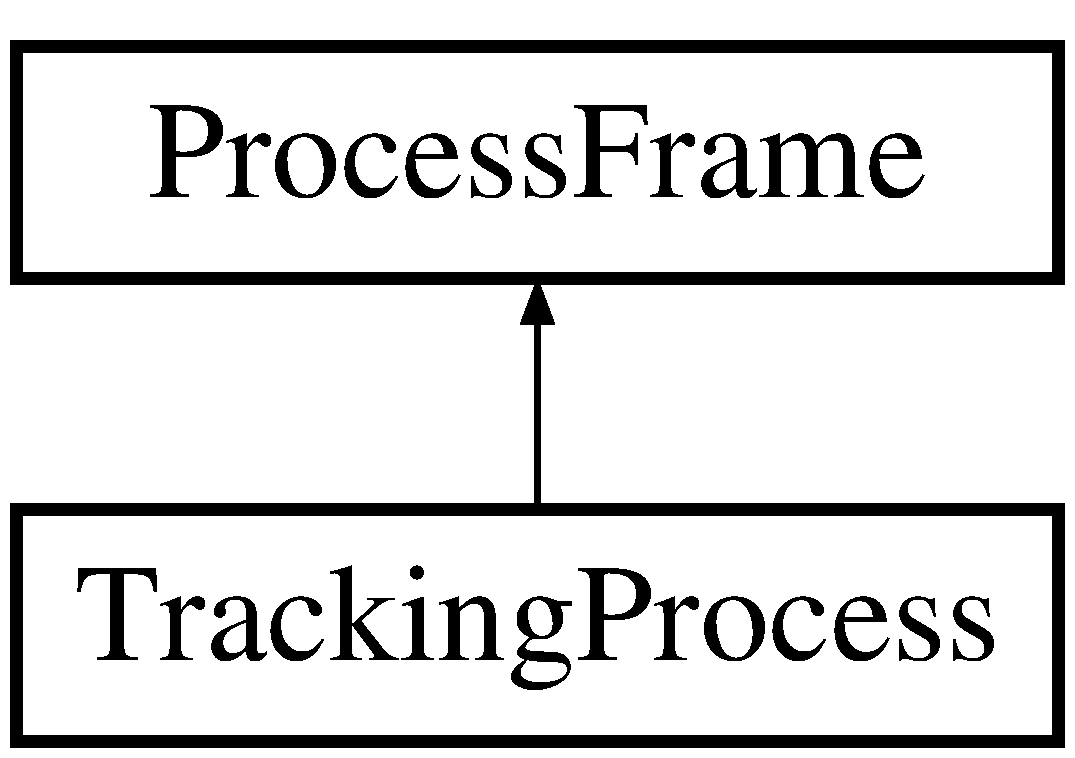
\includegraphics[height=2.000000cm]{class_tracking_process}
\end{center}
\end{figure}
\subsection*{Public Member Functions}
\begin{DoxyCompactItemize}
\item 
\hyperlink{class_tracking_process_a155da76d3cde928fb05e15de76c93640}{Tracking\+Process} (const Ptr$<$ \hyperlink{class_tracker}{Tracker} $>$ \&trk, const vector$<$ vector$<$ Point2f $>$ $>$ \&gt)
\item 
void \hyperlink{class_tracking_process_a8e10ca81e6df17389e1bdd7cec852613}{set\+Tracker} (const Ptr$<$ \hyperlink{class_tracker}{Tracker} $>$ \&trk)
\item 
void \hyperlink{class_tracking_process_a648f36431e7c0932b4befec1fdbc7e44}{left\+Button\+Down} (int x, int y, int flags)
\item 
void \hyperlink{class_tracking_process_a4d1f2b19eda65a24a301ab28e3c56fe2}{mouse\+Move} (int x, int y, int flags)
\item 
void \hyperlink{class_tracking_process_aa4622c0d0e0f4968fc67b414d5989b25}{operator()} (const size\+\_\+t frameN, const Mat \&frame, Mat \&output)
\end{DoxyCompactItemize}


\subsection{Detailed Description}
\hyperlink{class_tracking_process}{Tracking\+Process} class Inherites from vivalib Process\+Frame class to define a functor class that is called each time an input frame is available form the sequence and also handles mouse and keyboard events. 

\subsection{Constructor \& Destructor Documentation}
\index{Tracking\+Process@{Tracking\+Process}!Tracking\+Process@{Tracking\+Process}}
\index{Tracking\+Process@{Tracking\+Process}!Tracking\+Process@{Tracking\+Process}}
\subsubsection[{\texorpdfstring{Tracking\+Process(const Ptr$<$ Tracker $>$ \&trk, const vector$<$ vector$<$ Point2f $>$ $>$ \&gt)}{TrackingProcess(const Ptr< Tracker > &trk, const vector< vector< Point2f > > &gt)}}]{\setlength{\rightskip}{0pt plus 5cm}Tracking\+Process\+::\+Tracking\+Process (
\begin{DoxyParamCaption}
\item[{const Ptr$<$ {\bf Tracker} $>$ \&}]{trk, }
\item[{const vector$<$ vector$<$ Point2f $>$ $>$ \&}]{gt}
\end{DoxyParamCaption}
)\hspace{0.3cm}{\ttfamily [inline]}}\hypertarget{class_tracking_process_a155da76d3cde928fb05e15de76c93640}{}\label{class_tracking_process_a155da76d3cde928fb05e15de76c93640}
Constructor of a tracking process \begin{DoxySeeAlso}{See also}
\hyperlink{class_tracker}{Tracker} 

\hyperlink{class_tracker_factory}{Tracker\+Factory} 
\end{DoxySeeAlso}

\begin{DoxyParams}{Parameters}
{\em trk} & \+: pointer to a \hyperlink{class_tracker}{Tracker} object. \\
\hline
{\em gt} & ground-\/truth defined as a 2D list points. The ground-\/truth area for frame number N can be found by gt\mbox{[}N\mbox{]}. \\
\hline
\end{DoxyParams}


\subsection{Member Function Documentation}
\index{Tracking\+Process@{Tracking\+Process}!left\+Button\+Down@{left\+Button\+Down}}
\index{left\+Button\+Down@{left\+Button\+Down}!Tracking\+Process@{Tracking\+Process}}
\subsubsection[{\texorpdfstring{left\+Button\+Down(int x, int y, int flags)}{leftButtonDown(int x, int y, int flags)}}]{\setlength{\rightskip}{0pt plus 5cm}void Tracking\+Process\+::left\+Button\+Down (
\begin{DoxyParamCaption}
\item[{int}]{x, }
\item[{int}]{y, }
\item[{int}]{flags}
\end{DoxyParamCaption}
)}\hypertarget{class_tracking_process_a648f36431e7c0932b4befec1fdbc7e44}{}\label{class_tracking_process_a648f36431e7c0932b4befec1fdbc7e44}
Override from Process\+Frame class in vivalib Handles mouse left clicks. Used to defined new rectangular selection areas in the displayed windows and intilialize the tracker. 
\begin{DoxyParams}{Parameters}
{\em x} & x-\/coordinate of the clicked pixel in the image \\
\hline
{\em y} & y-\/coordinate of the clicked pixel in the image \\
\hline
{\em flags} & Open\+CV flags for mouse clicks \\
\hline
\end{DoxyParams}
\index{Tracking\+Process@{Tracking\+Process}!mouse\+Move@{mouse\+Move}}
\index{mouse\+Move@{mouse\+Move}!Tracking\+Process@{Tracking\+Process}}
\subsubsection[{\texorpdfstring{mouse\+Move(int x, int y, int flags)}{mouseMove(int x, int y, int flags)}}]{\setlength{\rightskip}{0pt plus 5cm}void Tracking\+Process\+::mouse\+Move (
\begin{DoxyParamCaption}
\item[{int}]{x, }
\item[{int}]{y, }
\item[{int}]{flags}
\end{DoxyParamCaption}
)}\hypertarget{class_tracking_process_a4d1f2b19eda65a24a301ab28e3c56fe2}{}\label{class_tracking_process_a4d1f2b19eda65a24a301ab28e3c56fe2}
Override from Process\+Frame class in vivalib Handles mouse movements over the displayed window. 
\begin{DoxyParams}{Parameters}
{\em x} & x-\/coordinate of the current location of the mouse in the displayed window \\
\hline
{\em y} & y-\/coordinate of the current location of the mouse in the displayed window \\
\hline
{\em flags} & Open\+CV flag \\
\hline
\end{DoxyParams}
\index{Tracking\+Process@{Tracking\+Process}!operator()@{operator()}}
\index{operator()@{operator()}!Tracking\+Process@{Tracking\+Process}}
\subsubsection[{\texorpdfstring{operator()(const size\+\_\+t frame\+N, const Mat \&frame, Mat \&output)}{operator()(const size_t frameN, const Mat &frame, Mat &output)}}]{\setlength{\rightskip}{0pt plus 5cm}void Tracking\+Process\+::operator() (
\begin{DoxyParamCaption}
\item[{const size\+\_\+t}]{frameN, }
\item[{const Mat \&}]{frame, }
\item[{Mat \&}]{output}
\end{DoxyParamCaption}
)}\hypertarget{class_tracking_process_aa4622c0d0e0f4968fc67b414d5989b25}{}\label{class_tracking_process_aa4622c0d0e0f4968fc67b414d5989b25}
Functor operator called each time that an input frame is available 
\begin{DoxyParams}{Parameters}
{\em frameN} & number of the frame \\
\hline
{\em frame} & the frame image \\
\hline
{\em output} & the processed tracking output image \\
\hline
\end{DoxyParams}
\index{Tracking\+Process@{Tracking\+Process}!set\+Tracker@{set\+Tracker}}
\index{set\+Tracker@{set\+Tracker}!Tracking\+Process@{Tracking\+Process}}
\subsubsection[{\texorpdfstring{set\+Tracker(const Ptr$<$ Tracker $>$ \&trk)}{setTracker(const Ptr< Tracker > &trk)}}]{\setlength{\rightskip}{0pt plus 5cm}void Tracking\+Process\+::set\+Tracker (
\begin{DoxyParamCaption}
\item[{const Ptr$<$ {\bf Tracker} $>$ \&}]{trk}
\end{DoxyParamCaption}
)}\hypertarget{class_tracking_process_a8e10ca81e6df17389e1bdd7cec852613}{}\label{class_tracking_process_a8e10ca81e6df17389e1bdd7cec852613}


The documentation for this class was generated from the following files\+:\begin{DoxyCompactItemize}
\item 
trackerlib/\hyperlink{tracking__process_8h}{tracking\+\_\+process.\+h}\item 
trackerlib/\hyperlink{tracking__process_8cpp}{tracking\+\_\+process.\+cpp}\end{DoxyCompactItemize}

\chapter{File Documentation}
\hypertarget{factories_8cpp}{}\section{trackerlib/factories.cpp File Reference}
\label{factories_8cpp}\index{trackerlib/factories.\+cpp@{trackerlib/factories.\+cpp}}
{\ttfamily \#include \char`\"{}factories.\+h\char`\"{}}\\*

\hypertarget{factories_8h}{}\section{trackerlib/factories.h File Reference}
\label{factories_8h}\index{trackerlib/factories.\+h@{trackerlib/factories.\+h}}
{\ttfamily \#include \char`\"{}precomp.\+h\char`\"{}}\\*
{\ttfamily \#include \char`\"{}tracking\+\_\+process.\+h\char`\"{}}\\*
\subsection*{Classes}
\begin{DoxyCompactItemize}
\item 
class \hyperlink{class_tracker_factory}{Tracker\+Factory}
\item 
class \hyperlink{class_ground_truth}{Ground\+Truth}
\end{DoxyCompactItemize}

\hypertarget{tracker_8h}{}\section{trackerlib/tracker.h File Reference}
\label{tracker_8h}\index{trackerlib/tracker.\+h@{trackerlib/tracker.\+h}}
{\ttfamily \#include $<$string$>$}\\*
{\ttfamily \#include \char`\"{}utils.\+h\char`\"{}}\\*
{\ttfamily \#include \char`\"{}opencv2/opencv.\+hpp\char`\"{}}\\*
\subsection*{Classes}
\begin{DoxyCompactItemize}
\item 
class \hyperlink{class_tracker}{Tracker}
\end{DoxyCompactItemize}

\hypertarget{tracking__process_8cpp}{}\section{trackerlib/tracking\+\_\+process.cpp File Reference}
\label{tracking__process_8cpp}\index{trackerlib/tracking\+\_\+process.\+cpp@{trackerlib/tracking\+\_\+process.\+cpp}}
{\ttfamily \#include \char`\"{}tracking\+\_\+process.\+h\char`\"{}}\\*

\hypertarget{tracking__process_8h}{}\section{trackerlib/tracking\+\_\+process.h File Reference}
\label{tracking__process_8h}\index{trackerlib/tracking\+\_\+process.\+h@{trackerlib/tracking\+\_\+process.\+h}}
{\ttfamily \#include \char`\"{}viva.\+h\char`\"{}}\\*
{\ttfamily \#include \char`\"{}tracker.\+h\char`\"{}}\\*
{\ttfamily \#include $<$fstream$>$}\\*
\subsection*{Classes}
\begin{DoxyCompactItemize}
\item 
class \hyperlink{class_rect_select_area}{Rect\+Select\+Area}
\item 
struct \hyperlink{struct_color}{Color}
\item 
class \hyperlink{class_tracking_process}{Tracking\+Process}
\item 
class \hyperlink{class_draw}{Draw}
\end{DoxyCompactItemize}

%--- End generated contents ---

% Index
\backmatter
\newpage
\phantomsection
\clearemptydoublepage
\addcontentsline{toc}{chapter}{Index}
\printindex

\end{document}
